\chapter{Cheating}

\section{Definition}
We define cheating as the following: If an aggregator changes the sensor readings reported by its children to skew the final aggregated result.

\section{Aim}
Aim of this section is to detect the cheater with given definition. 

\section{Assumptions}
We make an assumption that the cheater can not say NACK during verification phase. If a cheater node is allowed to send NACK message then it can send NACK messages all the time and create a lot of traffic in the network which might create Denial of service attack. 

\section{What is not cheating ?}
	
	In figure 7.1, A is an aggregator if A wants to skew the final aggregation result it can do it. No matter what B's sensor reading is A can adjust its sensor readin to meat the final requirement. 
	We do not consider this case as a cheating because A is adjusting its sensor reading, it's not changing the B's sensor reading. 
  
	\begin{figure}[t]
		\centering
			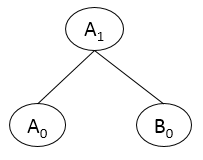
\includegraphics[width=0.2\textwidth]{commitment_tree_1.png}\\
			\caption{Possible commitment tree}
		\label{fig:figure2}
	\end{figure}

	Similar arguments can be done for figure 7.3 if A, C  both are cheaters. In that case A is adjusting C's sensor reading to skew the final aggregation result and C will not complain as it is a cheater.

	\begin{figure}[t]
		\centering
			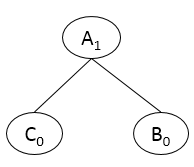
\includegraphics[width=0.2\textwidth]{commitment_tree_2.png}
			\caption{Possible commitment tree}
		\label{fig:figure2}
	\end{figure}

\section{Detecting a cheater}
	
	In figure 7.3,

	Case I: A says NACK during verification phase
	Implies I: I is a cheater.

	Case I: A, B says NACK during verification phase
	Implies I: Either I or M is a cheater. 
	

	If d = depth of a tree,\\

	\begin{tabular}{| l | l |}
    \hline
    Depth of a cheater & Minimum number of complains \\ \hline
    d - 1 & 1 \\ \hline
    d - 2 & 2 \\ \hline
    d - 3 & 4 \\ \hline
    d - 4 & 8 \\ \hline
    \end{tabular}

	\begin{figure}[t]
		\centering
			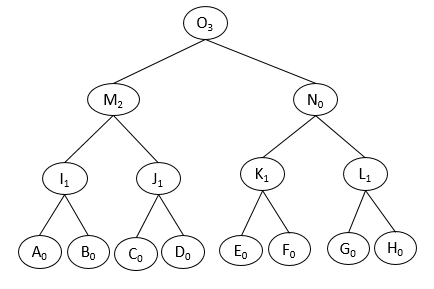
\includegraphics[width=0.8\textwidth]{commitment_tree_3.png}
			\caption{Possible commitment tree}
		\label{fig:figure2}
	\end{figure}